% !TEX program = xelatex
% Supplementary Information (English only)
% Compile: xelatex supplementary_information_en.tex
\documentclass[11pt,a4paper]{article}

\usepackage[margin=2.4cm]{geometry}
\usepackage{amsmath,amssymb}
\usepackage{graphicx}
\usepackage{setspace}
\usepackage{parskip}
\usepackage{titlesec}
\usepackage{booktabs}
\usepackage{tabularx}
\usepackage{multirow}
\usepackage{hyperref}
\usepackage{xcolor}
\usepackage{caption}
\usepackage{longtable}
\usepackage{array}
\usepackage{fontspec}

\setmainfont{Times New Roman}

\titleformat{\section}{\normalfont\large\bfseries}{\thesection}{0.6em}{}
\titleformat{\subsection}{\normalfont\normalsize\bfseries}{\thesubsection}{0.5em}{}

\setlength{\parskip}{0.6em}
\setlength{\parindent}{0pt}
\onehalfspacing

% Figure path
\graphicspath{{../../0414_v4/figures/}}

% Convenience macros
\newcommand{\keff}{\ensuremath{k_{\mathrm{eff}}}}
\newcommand{\Eint}{\ensuremath{E_{\mathrm{intercept}}}}
\newcommand{\Eslope}{\ensuremath{E_{\mathrm{slope}}}}
\newcommand{\abase}{\ensuremath{\alpha_{\mathrm{base}}}}
\newcommand{\aslope}{\ensuremath{\alpha_{\mathrm{slope}}}}
\newcommand{\kref}{\ensuremath{k_{\mathrm{ref}}}}
\newcommand{\Tref}{\ensuremath{T_{\mathrm{ref}}}}
\newcommand{\kslope}{\ensuremath{k_{\mathrm{slope}}}}

\title{\textbf{Supplementary Information}\\[0.3em]
\large Bayesian Neural Surrogates Unify Uncertainty Propagation,\\
Sensitivity Attribution and Calibration for Coupled\\
Multi-Physics Reactor Analysis}
\author{Yinuo Chen, Sicheng Wang, Xiaojing Liu*, Tengfei Zhang*}
\date{}

\begin{document}
\maketitle

\tableofcontents
\newpage

% ======================================================================
\section{Supplementary Figures}
\label{sec:figures}
% ======================================================================

% --- Fig. S1 ---
\begin{figure}[htbp]
\centering
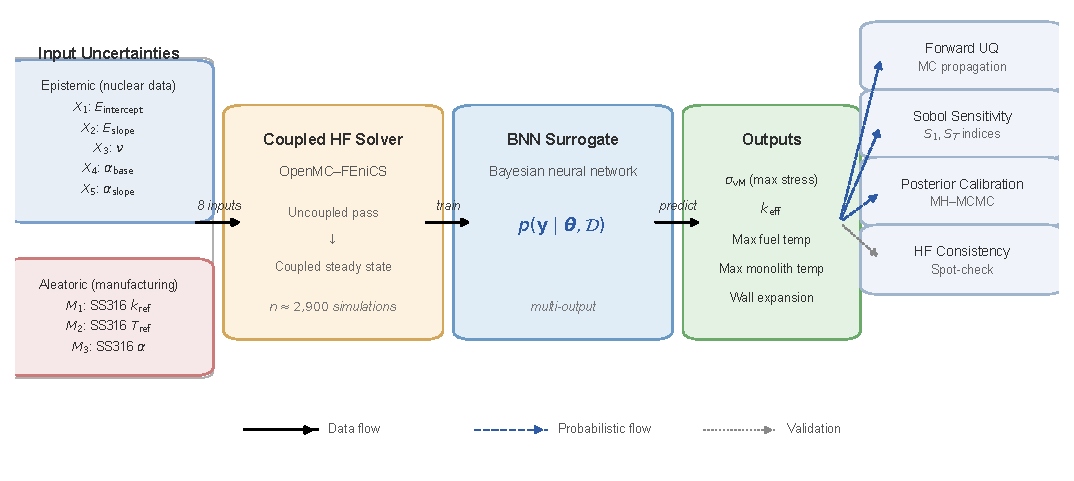
\includegraphics[width=\textwidth]{fig0_workflow.pdf}
\caption{\textbf{Fig.~S1~|~BNN surrogate workflow.}
Schematic of the end-to-end probabilistic analysis framework. The BNN
surrogate is trained on coupled OpenMC--FEniCS data and produces a
posterior predictive distribution. This single distribution serves as
the shared probabilistic layer for forward uncertainty propagation,
Sobol sensitivity attribution, and MCMC posterior calibration, without
retraining between analyses.}
\label{fig:S1}
\end{figure}

% --- Fig. S2 ---
\begin{figure}[htbp]
\centering
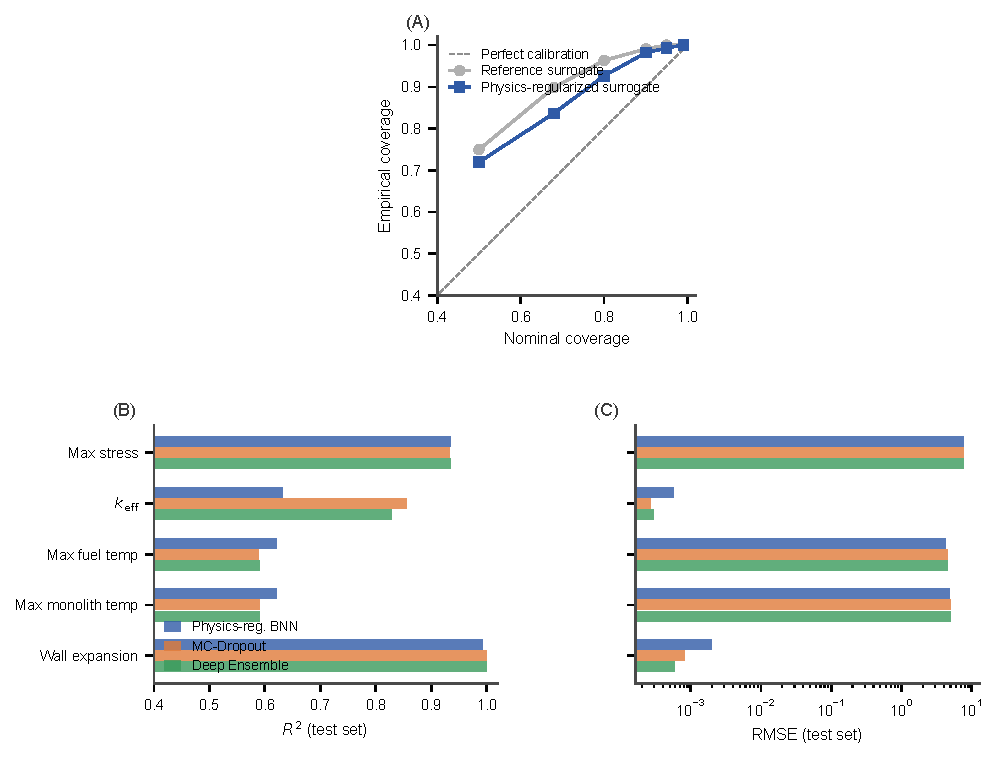
\includegraphics[width=\textwidth]{figA1_model_validation.pdf}
\caption{\textbf{Fig.~S2~|~Model validation: parity and residual analysis.}
Predicted versus true values and residual distributions for primary
outputs across all four BNN variants (435 test samples). Shaded regions
show the 90\% predictive interval.}
\label{fig:S2}
\end{figure}

% --- Fig. S3 ---
\begin{figure}[htbp]
\centering
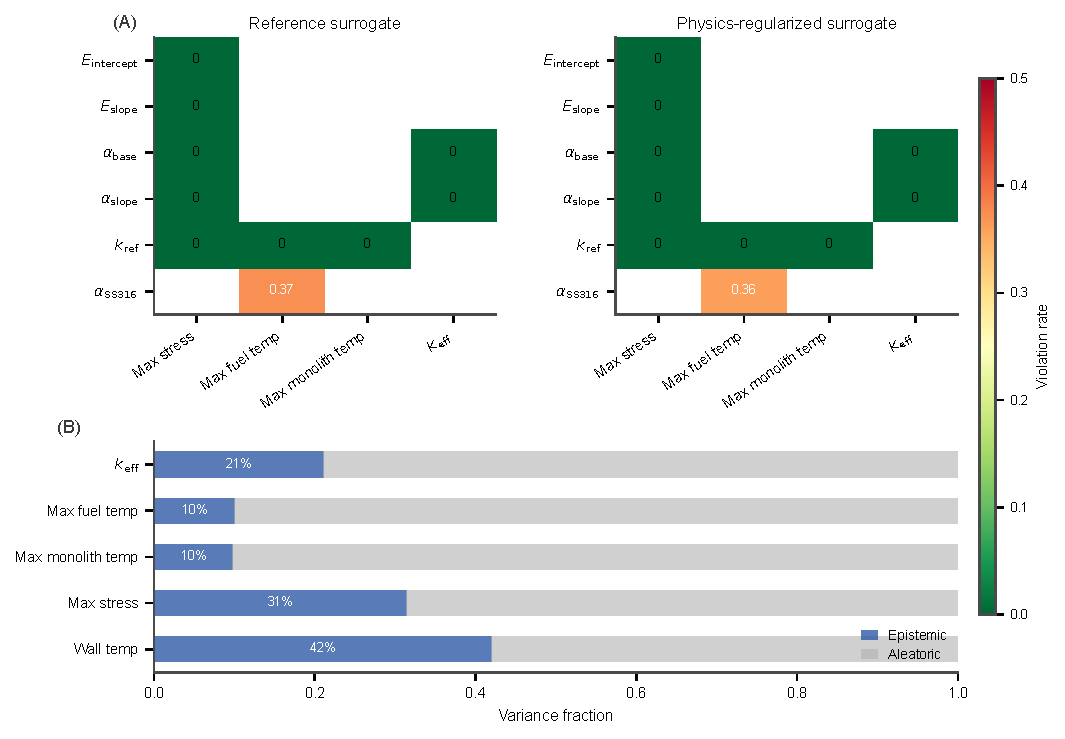
\includegraphics[width=\textwidth]{figA2_physics_robustness.pdf}
\caption{\textbf{Fig.~S3~|~Physics consistency and uncertainty decomposition.}
(\textbf{A})~Monotonicity violation rates for 15 input--output pairs
across four BNN variants; high-confidence pairs achieve zero violations.
(\textbf{B})~Epistemic vs.\ aleatoric variance decomposition. Aleatoric
uncertainty dominates across all outputs (58--90\% of total variance).}
\label{fig:S3}
\end{figure}

% --- Fig. S4 ---
\begin{figure}[htbp]
\centering
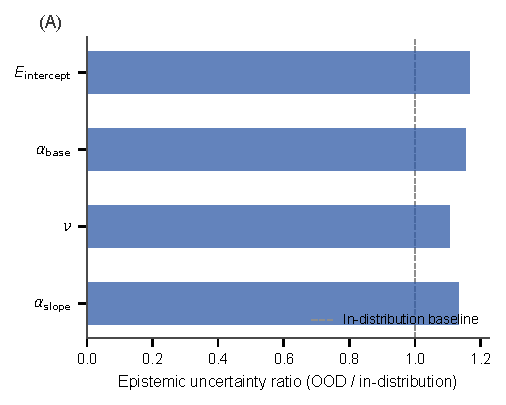
\includegraphics[width=\textwidth]{figS4_ood.pdf}
\caption{\textbf{Fig.~S4~|~Out-of-distribution (OOD) coverage and
epistemic uncertainty.}
90\% predictive interval coverage for in-distribution versus four
feature-tail subsets. Stress retains coverage above 0.75 across all
tails. \keff{} coverage degrades substantially on the \abase{} tail
($R^2$ drops to approximately 0.29), indicating that the Sobol and
posterior conclusions for \keff{} are valid only within the training
range of this dominant parameter. Elevated epistemic ratios on the
\abase{} tail confirm that the BNN correctly signals increased model
uncertainty outside the training domain.}
\label{fig:S4}
\end{figure}

% --- Fig. S5 ---
\begin{figure}[htbp]
\centering
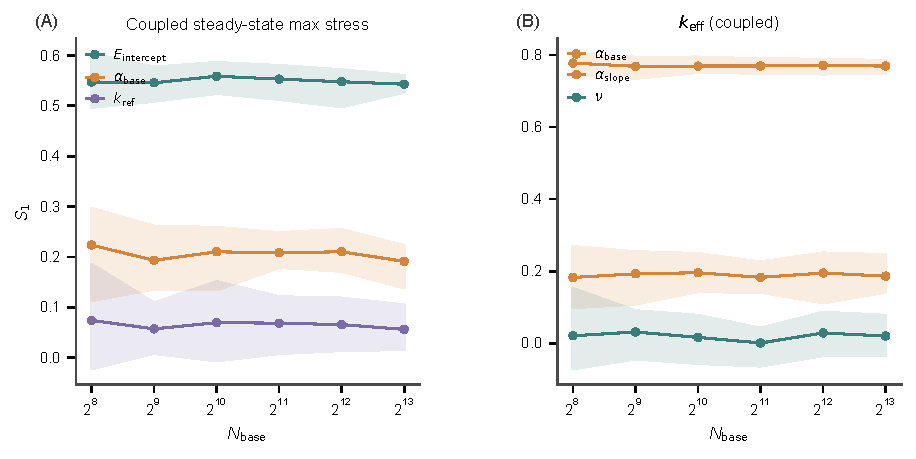
\includegraphics[width=\textwidth]{figS1_sobol_convergence.pdf}
\caption{\textbf{Fig.~S5~|~Sobol index convergence with sample size.}
First-order Sobol index $S_1$ as a function of sample size $N_S$
(256 to 4096) for stress and \keff{}, with 90\% CI bands across
50 replications. Indices stabilise by $N_S = 2048$, confirming
convergence at the chosen $N_S = 4096$.}
\label{fig:S5}
\end{figure}

% --- Fig. S6 ---
\begin{figure}[htbp]
\centering
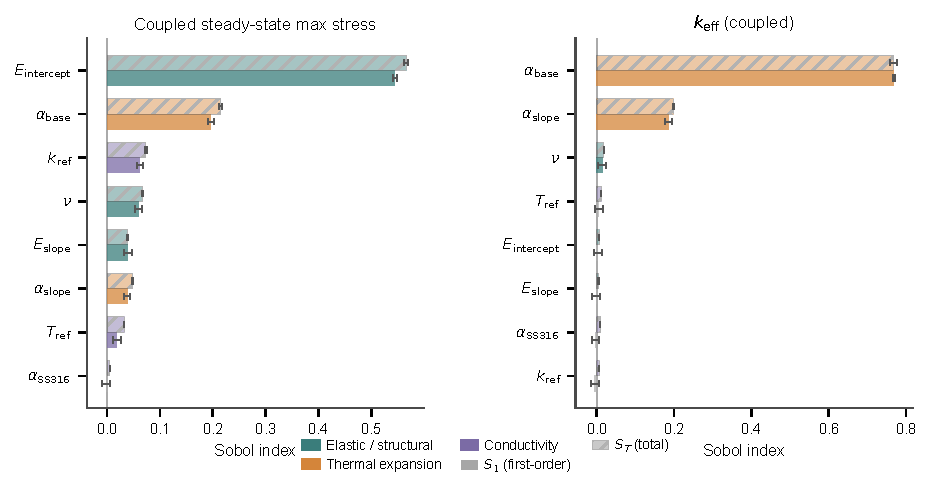
\includegraphics[width=\textwidth]{figA4_sobol_detail.pdf}
\caption{\textbf{Fig.~S6~|~Detailed Sobol sensitivity analysis.}
First-order and total-order Sobol indices for all eight material
parameters across all five primary outputs, showing the dominance
of \Eint{} for stress and \abase{} for \keff{}.}
\label{fig:S6}
\end{figure}

% --- Fig. S7 ---
\begin{figure}[htbp]
\centering
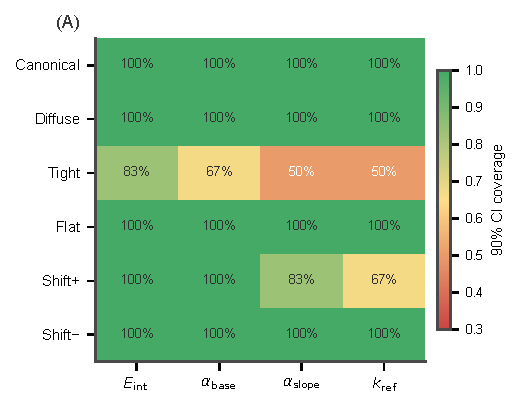
\includegraphics[width=\textwidth]{figS2_prior_sensitivity.pdf}
\caption{\textbf{Fig.~S7~|~Prior sensitivity analysis.}
Posterior marginal distributions for the four calibrated parameters
under six prior configurations: canonical, diffuse ($2\times$), tight
($0.5\times$), flat (uniform), shift$_{+}$ ($\mu + 0.5\sigma$),
shift$_{-}$ ($\mu - 0.5\sigma$). The tight prior over-constrains the
posterior, reducing coverage to 50--83\% (Table~S10).}
\label{fig:S7}
\end{figure}

% --- Fig. S8 ---
\begin{figure}[htbp]
\centering
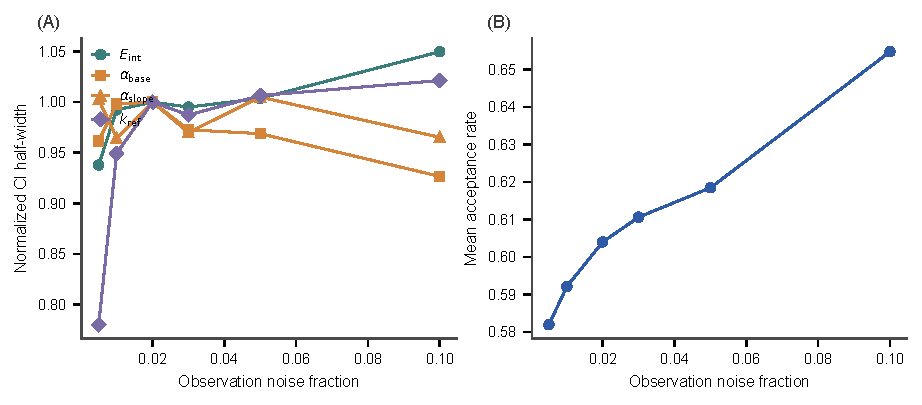
\includegraphics[width=\textwidth]{figS3_noise_sensitivity.pdf}
\caption{\textbf{Fig.~S8~|~Observation noise sensitivity.}
Posterior width and acceptance rate as a function of assumed observation
noise fraction (0.5\%--10\%). Posterior standard deviations increase
monotonically; acceptance rates increase appropriately as the likelihood
broadens (Table~S11).}
\label{fig:S8}
\end{figure}

% --- Fig. S9 ---
\begin{figure}[htbp]
\centering
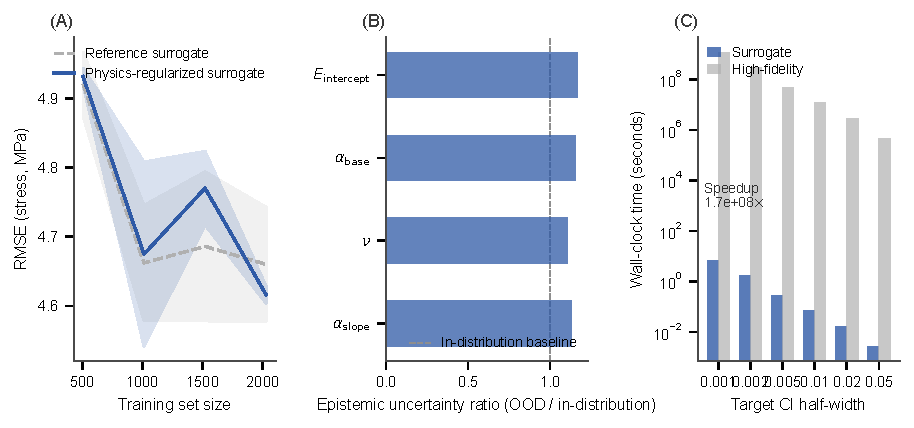
\includegraphics[width=\textwidth]{figA3_efficiency.pdf}
\caption{\textbf{Fig.~S9~|~Data efficiency and computational cost.}
Test RMSE and $R^2$ as a function of training set size for the
physics-regularized BNN. Near-saturated performance is achieved at
25\% data utilisation (507 training samples; Table~S12).}
\label{fig:S9}
\end{figure}

% --- Fig. S10 ---
\begin{figure}[htbp]
\centering
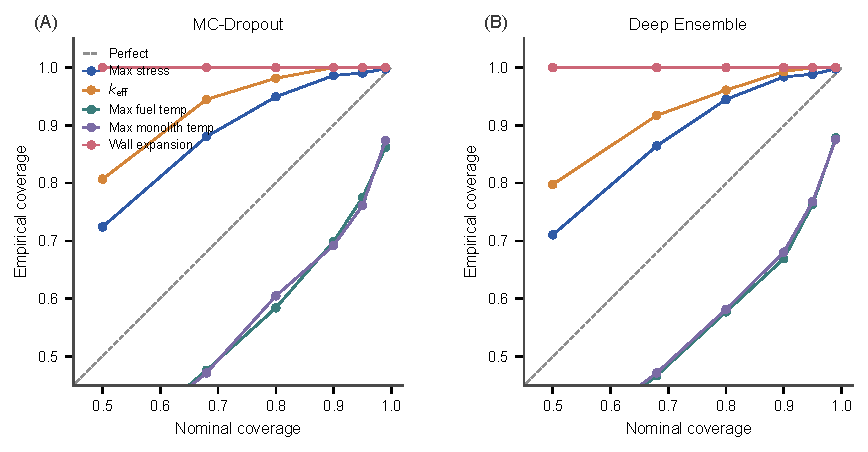
\includegraphics[width=\textwidth]{figS5_external_calib.pdf}
\caption{\textbf{Fig.~S10~|~External baseline calibration comparison.}
Calibration curves comparing BNN, MC-Dropout and deep ensemble across
primary outputs. The BNN achieves substantially better probabilistic
calibration (ECE 0.027 vs.\ 0.18--0.19) on temperature outputs.}
\label{fig:S10}
\end{figure}

\clearpage

% ======================================================================
\section{Supplementary Tables}
\label{sec:tables}
% ======================================================================

% --- Table S1 ---
\begin{table}[htbp]
\centering
\caption{\textbf{Table~S1~|~Material parameters: definitions, nominal values
and priors.}}
\label{tab:S1}
\smallskip
\small
\begin{tabular}{lllll}
\toprule
Parameter & Symbol & Nominal value & Unit & Prior range ($\pm$10\%) \\
\midrule
Young's mod.\ intercept & \Eint{} & $2\times10^{11}$ & Pa
  & $[1.8, 2.2]\times10^{11}$ \\
Young's mod.\ slope & \Eslope{} & $-7\times10^{7}$ & Pa/K
  & $[-7.7, -6.3]\times10^{7}$ \\
Poisson's ratio & $\nu$ & 0.31 & ---
  & [0.279, 0.341] \\
CTE base & \abase{} & $1\times10^{-5}$ & K$^{-1}$
  & $[0.9, 1.1]\times10^{-5}$ \\
CTE slope & \aslope{} & $5\times10^{-9}$ & K$^{-2}$
  & $[4.5, 5.5]\times10^{-9}$ \\
Ref.\ conductivity & \kref{} & 23.2 & W/(m$\cdot$K)
  & [20.88, 25.52] \\
Ref.\ temperature & \Tref{} & 923.15 & K
  & [830.84, 1015.47] \\
Cond.\ slope & \kslope{} & 1/75 & W/(m$\cdot$K$^2$)
  & [0.012, 0.0147] \\
\bottomrule
\end{tabular}
\end{table}

% --- Table S2 ---
\begin{table}[htbp]
\centering
\caption{\textbf{Table~S2~|~BNN hyperparameter search space and optimal
values.}}
\label{tab:S2}
\smallskip
\small
\begin{tabular}{lll}
\toprule
Hyperparameter & Search range & Optimal (bnn-phy-mono) \\
\midrule
Width           & [64, 256]           & 254 \\
Depth           & [2, 8]              & 2 \\
Learning rate   & [$10^{-4}$, $10^{-2}$] & $9.81\times10^{-4}$ \\
Weight decay    & [$10^{-9}$, $10^{-5}$] & $8.09\times10^{-8}$ \\
Batch size      & \{16, 32, 64\}      & 32 \\
Epochs          & [200, 500]          & 399 \\
Gradient clip   & [0.1, 2.0]          & 0.674 \\
$w_\mathrm{data}$ & [0.1, 5.0]       & 1.855 \\
Prior $\sigma$  & [0.1, 2.0]          & 0.478 \\
KL weight       & [$10^{-5}$, $10^{-2}$] & $1.93\times10^{-4}$ \\
$w_\mathrm{mono}$ & [0.01, 1.0]      & 0.212 \\
$\rho_\mathrm{abs,min}$ & [0.01, 0.5] & 0.123 \\
mono\_topk      & [10, 100]           & 53 \\
\bottomrule
\end{tabular}

\smallskip
Search: Optuna with 200 trials; objective: validation RMSE.
Activation: SiLU throughout. Output heads: mean + log-variance
(heteroscedastic).
\end{table}

% --- Table S3 ---
\begin{table}[htbp]
\centering
\caption{\textbf{Table~S3~|~BNN ablation study: four model variants on
five primary outputs} (mean $\pm$ s.d., 5 seeds).}
\label{tab:S3}
\smallskip
\small
\begin{tabular}{lccc}
\toprule
Model variant & Stress $R^2$ & Stress PICP & \keff{} $R^2$ \\
\midrule
Reference (ELBO only) & $0.936\pm0.007$ & $0.995\pm0.002$ & $0.633\pm0.260$ \\
Data-monotone         & $0.932\pm0.005$ & $0.998\pm0.002$ & $0.635\pm0.260$ \\
Physics-regularized   & $0.935\pm0.007$ & $0.987\pm0.007$ & $0.633\pm0.258$ \\
Data+inequality       & $0.924\pm0.007$ & $1.000\pm0.001$ & $0.617\pm0.249$ \\
\bottomrule
\end{tabular}
\end{table}

% --- Table S4 ---
\begin{table}[htbp]
\centering
\caption{\textbf{Table~S4~|~Complete Sobol indices ($S_1$ and $S_T$) for
stress and \keff{}} (physics-regularized BNN, $N_S = 4096$,
50 replications, 90\% CI).}
\label{tab:S4}
\smallskip
\small
\begin{tabular}{lcc}
\toprule
Parameter & Stress $S_1$ [90\% CI] & Stress $S_T$ [90\% CI] \\
\midrule
\Eslope{}    & 0.037 [$-$0.046, 0.100] & 0.039 [0.038, 0.039] \\
\Eint{}      & 0.548 [0.498, 0.572]    & 0.566 [0.562, 0.571] \\
$\nu$        & 0.063 [0.034, 0.097]    & 0.068 [0.067, 0.069] \\
\abase{}     & 0.210 [0.171, 0.254]    & 0.214 [0.212, 0.217] \\
\aslope{}    & 0.038 [$-$0.013, 0.091] & 0.047 [0.046, 0.049] \\
\Tref{}      & 0.019 [$-$0.025, 0.055] & 0.032 [0.031, 0.033] \\
\kref{}      & 0.065 [0.014, 0.118]    & 0.073 [0.072, 0.075] \\
SS316\_$\alpha$ & $-$0.004 [$-$0.068, 0.034] & 0.005 [0.005, 0.006] \\
\midrule
Parameter & \keff{} $S_1$ [90\% CI] & \keff{} $S_T$ [90\% CI] \\
\midrule
\Eslope{}    & 0.010 [$-$0.052, 0.062] & 0.005 [0.004, 0.005] \\
\Eint{}      & 0.008 [$-$0.065, 0.071] & 0.006 [0.006, 0.007] \\
$\nu$        & 0.029 [$-$0.035, 0.086] & 0.018 [0.018, 0.019] \\
\abase{}     & 0.771 [0.747, 0.788]    & 0.767 [0.758, 0.776] \\
\aslope{}    & 0.195 [0.112, 0.250]    & 0.198 [0.196, 0.201] \\
\Tref{}      & 0.010 [$-$0.023, 0.054] & 0.011 [0.011, 0.012] \\
\kref{}      & 0.000 [$-$0.063, 0.048] & 0.006 [0.006, 0.007] \\
SS316\_$\alpha$ & 0.003 [$-$0.059, 0.074] & 0.009 [0.009, 0.009] \\
\bottomrule
\end{tabular}
\end{table}

% --- Table S5 ---
\begin{table}[htbp]
\centering
\caption{\textbf{Table~S5~|~Posterior calibration: 18 benchmark case
summary} (physics-regularized BNN).}
\label{tab:S5}
\smallskip
\small
\begin{tabular}{clcccc}
\toprule
Case & Category & True stress (MPa) & Accept rate & 90\%-CI coverage & Post-mean err. \\
\midrule
 0 & low  & 110.6 & 0.619 & 3/4 &  8.3 \\
 1 & low  & 118.7 & 0.612 & 4/4 & 24.6 \\
 2 & low  & 110.7 & 0.620 & 2/4 &  9.0 \\
 3 & low  & 103.7 & 0.618 & 4/4 &  8.8 \\
 4 & low  & 114.5 & 0.621 & 4/4 &  3.1 \\
 5 & low  & 102.0 & 0.616 & 3/4 & 23.4 \\
 6 & near & 127.6 & 0.609 & 4/4 & 20.3 \\
 7 & near & 127.9 & 0.586 & 4/4 & 26.6 \\
 8 & near & 127.0 & 0.611 & 4/4 &  5.9 \\
 9 & near & 123.5 & 0.613 & 4/4 &  3.5 \\
10 & near & 128.9 & 0.609 & 3/4 &  4.5 \\
11 & near & 129.3 & 0.610 & 4/4 &  3.8 \\
12 & high & 169.5 & 0.592 & 4/4 &  0.2 \\
13 & high & 176.0 & 0.591 & 4/4 & 12.1 \\
14 & high & 193.4 & 0.598 & 3/4 & 13.7 \\
15 & high & 163.4 & 0.591 & 4/4 &  3.6 \\
16 & high & 142.8 & 0.582 & 4/4 & 10.5 \\
17 & high & 197.6 & 0.583 & 4/4 &  5.4 \\
\midrule
\multicolumn{2}{l}{Overall} & & 0.58--0.62 & 66/72 = 0.917 & MAE = 10.4 \\
\bottomrule
\end{tabular}
\end{table}

% --- Table S6 ---
\begin{table}[htbp]
\centering
\caption{\textbf{Table~S6~|~Computational cost breakdown.}}
\label{tab:S6}
\smallskip
\small
\begin{tabular}{lll}
\toprule
Operation & Time & Platform \\
\midrule
Coupled HF solve (1 case) & 2266\,s & EPYC 9654 / 96 cores \\
BNN single draw ($M=50$) & $1.29\times10^{-2}$\,s & GPU \\
BNN batched (batch=1024, per sample) & $1.34\times10^{-5}$\,s & GPU \\
20,000-sample forward UQ & ${\sim}0.3$\,s & GPU \\
Sobol (50 reps $\times$ 40,960 evals) & ${\sim}$minutes & GPU \\
18-case MCMC (8000 iter $\times$ 4 chains) & ${\sim}$minutes & GPU \\
\midrule
Speedup (single draw vs.\ HF) & $1.76\times10^{5}$ & \\
Speedup (batched vs.\ HF) & $1.69\times10^{8}$ & \\
\bottomrule
\end{tabular}
\end{table}

% --- Table S7 ---
\begin{table}[htbp]
\centering
\caption{\textbf{Table~S7~|~Physics consistency: monotonicity violation
rates} (435 test samples, discrete $\pm\delta$ perturbation test).}
\label{tab:S7}
\smallskip
\small
\begin{tabular}{lcccc}
\toprule
Physics pair (input $\to$ output, sign) & Ref.\ BNN & Data-mono & Phy-reg & Data+ineq \\
\midrule
\Eint{} $\to$ Max stress (+)     & 0\% & 0\% & 0\% & 0\% \\
\abase{} $\to$ Max stress (+)    & 0\% & 0\% & 0\% & 0\% \\
\abase{} $\to$ \keff{} ($-$)     & 0\% & 0\% & 0\% & 0\% \\
\kref{} $\to$ Max stress ($-$)   & 0\% & 0\% & 0\% & 1.1\% \\
SS316\_$\alpha$ $\to$ Fuel temp ($-$) & 36.3\% & 39.5\% & 35.6\% & 53.6\% \\
\bottomrule
\end{tabular}

\smallskip
Inequality constraints (max $\geq$ average temp, stress $\geq 0$):
0\% violations for all four BNN variants.
\end{table}

% --- Table S8 ---
\begin{table}[htbp]
\centering
\caption{\textbf{Table~S8~|~Epistemic vs.\ aleatoric uncertainty
decomposition on test set.}}
\label{tab:S8}
\smallskip
\small
\begin{tabular}{lcccc}
\toprule
 & \multicolumn{2}{c}{Ref.\ BNN} & \multicolumn{2}{c}{Phy-reg BNN} \\
Output & Epi\% & Ale\% & Epi\% & Ale\% \\
\midrule
\keff{}            & 12.0 & 88.0 & 10.2 & 89.8 \\
Max fuel temp      & 12.0 & 88.0 & 10.1 & 89.9 \\
Max monolith temp  & 11.2 & 88.8 & 10.1 & 89.9 \\
Max stress         & 27.7 & 72.3 & 29.6 & 70.4 \\
Wall expansion     & 34.1 & 65.9 & 41.7 & 58.3 \\
\bottomrule
\end{tabular}
\end{table}

% --- Table S9 ---
\begin{table}[htbp]
\centering
\caption{\textbf{Table~S9~|~External baseline: full comparison of scoring
rules.}}
\label{tab:S9}
\smallskip
\small
\begin{tabular}{llccccc}
\toprule
Model & Output & RMSE & $R^2$ & CRPS & NLL & ECE \\
\midrule
MC-Dropout & \keff{} & 0.0003 & 0.856 & 0.0002 & $-$6.502 & 0.152 \\
           & Fuel temp   & 4.497 & 0.590 & 2.624 & 3.352 & 0.183 \\
           & Monolith T  & 5.061 & 0.590 & 2.951 & 3.472 & 0.182 \\
           & Max stress  & 7.659 & 0.934 & 4.519 & 3.592 & 0.118 \\
           & Wall exp.   & 0.0008 & 0.999 & 0.002 & $-$3.831 & 0.197 \\
\midrule
Deep Ensemble & \keff{} & 0.0003 & 0.828 & 0.0002 & $-$6.476 & 0.142 \\
              & Fuel temp   & 4.495 & 0.590 & 2.634 & 3.326 & 0.190 \\
              & Monolith T  & 5.061 & 0.590 & 2.962 & 3.439 & 0.185 \\
              & Max stress  & 7.644 & 0.934 & 4.502 & 3.586 & 0.112 \\
              & Wall exp.   & 0.0006 & 0.999 & 0.002 & $-$3.841 & 0.197 \\
\bottomrule
\end{tabular}
\end{table}

% --- Table S10 ---
\begin{table}[htbp]
\centering
\caption{\textbf{Table~S10~|~Prior sensitivity} (6 configurations,
physics-regularized BNN, case 06, near-threshold).}
\label{tab:S10}
\smallskip
\small
\begin{tabular}{lccc}
\toprule
Prior variant & Coverage (4 params) & Mean KL vs.\ canonical & Accept rate \\
\midrule
Canonical         & 100\%      & 0.00 (reference) & 0.61 \\
Diffuse ($2\times$)  & 100\%   & 0.15--0.22       & 0.63 \\
Tight ($0.5\times$)  & 50--83\% & 0.64--1.28      & 0.57 \\
Flat (uniform)    & 100\%      & 0.24--0.38       & 0.64 \\
Shift ($+0.5\sigma$) & 67--100\% & 0.06--0.36    & 0.60 \\
Shift ($-0.5\sigma$) & 83--100\% & 0.08--0.28    & 0.61 \\
\bottomrule
\end{tabular}
\end{table}

% --- Table S11 ---
\begin{table}[htbp]
\centering
\caption{\textbf{Table~S11~|~Noise sensitivity} (noise fraction
0.5\%--10\%, physics-regularized BNN, case 06).}
\label{tab:S11}
\smallskip
\small
\begin{tabular}{lccc}
\toprule
Noise fraction & \Eint{} post.\ std & Accept rate & Coverage \\
\midrule
0.5\%            & $1.26\times10^{10}$ & 0.58 & 100\% \\
1.0\%            & $1.28\times10^{10}$ & 0.59 & 100\% \\
2.0\% (default)  & $1.32\times10^{10}$ & 0.61 & 100\% \\
5.0\%            & $1.36\times10^{10}$ & 0.63 & 100\% \\
10.0\%           & $1.40\times10^{10}$ & 0.65 &  83\% \\
\bottomrule
\end{tabular}
\end{table}

% --- Table S12 ---
\begin{table}[htbp]
\centering
\caption{\textbf{Table~S12~|~Data efficiency} (2 seeds per fraction).}
\label{tab:S12}
\smallskip
\small
\begin{tabular}{lccc}
\toprule
Train fraction & $N_\mathrm{train}$ & RMSE (mean $\pm$ s.d.) & $R^2$ (mean $\pm$ s.d.) \\
\midrule
25\%  &  507 & $4.93\pm0.04$ & $0.768\pm0.002$ \\
50\%  & 1015 & $4.66\pm0.11$ & $0.782\pm0.005$ \\
75\%  & 1522 & $4.68\pm0.01$ & $0.784\pm0.002$ \\
100\% & 2029 & $4.62\pm0.08$ & $0.783\pm0.005$ \\
\bottomrule
\end{tabular}
\end{table}

\clearpage

% ======================================================================
\section{Supplementary Notes}
\label{sec:notes}
% ======================================================================

\subsection{Note A: BNN training details}

\subsubsection*{A.1.~Evidence lower bound (ELBO) derivation}

The BNN posterior over weights $\mathbf{w}$ is approximated by a
mean-field variational distribution
$q(\mathbf{w}) = \prod_i \mathcal{N}(w_i \mid \mu_i, \sigma_i^2)$.
The variational parameters are optimised by minimising the negative
evidence lower bound:
\begin{equation}
\mathcal{L}(\boldsymbol{\mu}, \boldsymbol{\sigma})
= \mathrm{KL}\bigl[q(\mathbf{w}) \,\|\, p(\mathbf{w})\bigr]
- \mathbb{E}_{q(\mathbf{w})}\bigl[\log p(\mathcal{D} \mid \mathbf{w})\bigr]
\end{equation}
where $p(\mathbf{w}) = \mathcal{N}(\mathbf{0}, \sigma_p^2 \mathbf{I})$
is the isotropic Gaussian prior. The KL divergence admits a closed form;
the data-fit term is approximated by a single Monte Carlo sample per
mini-batch (Bayes-by-Backprop\textsuperscript{10}).

The reparameterisation trick enables gradient computation:
$w = \mu + \sigma \cdot \epsilon$, where
$\epsilon \sim \mathcal{N}(0, \mathbf{I})$. The variance parameter
$\sigma = \log(1 + \exp(\rho))$ ensures positivity, with
$\rho_\mathrm{abs,min}$ clamping $\rho \geq \rho_\mathrm{abs,min}$
to prevent posterior collapse.

\subsubsection*{A.2.~Heteroscedastic observation noise}

The network outputs both a mean $\mu(\boldsymbol{\theta})$ and a
log-variance $\log \sigma^2_\mathrm{obs}(\boldsymbol{\theta})$ per
output channel:
\begin{equation}
\log p(y_j \mid \boldsymbol{\theta}, \mathbf{w})
= -\tfrac{1}{2}\bigl[\log \sigma^2_{\mathrm{obs},j}
+ (y_j - \mu_j)^2 / \sigma^2_{\mathrm{obs},j}\bigr]
\end{equation}
This heteroscedastic formulation allows the BNN to model
input-dependent observation noise, separating it from epistemic
(weight) uncertainty.

\subsubsection*{A.3.~KL annealing schedule}

The KL weight $\beta$ is annealed from 0 to its target value
$\mathrm{kl\_weight} = 1.93\times10^{-4}$ over the first 100 epochs:
$\beta(t) = \min(t/100, 1) \cdot \mathrm{kl\_weight}$.
This prevents the KL term from dominating early training before the
data-fit term has found a reasonable region of weight space.

\subsubsection*{A.4.~Physics-prior monotonicity constraints}

The physics-regularized BNN adds an auxiliary loss:
\begin{equation}
\mathcal{L}_\mathrm{mono}
= \frac{1}{K}\sum_{k=1}^{K}\max\bigl(0,\;
  -\mathrm{sign}\cdot\partial\mu/\partial\theta_k\bigr)
\end{equation}
weighted by $w_\mathrm{mono} = 0.212$. Sign constraints are derived
from constitutive physics---for example, stress increases with \Eint{}
because $\sigma = \mathbf{C}(E, \nu) \cdot \boldsymbol{\epsilon}$ and
$\mathbf{C}$ is linear in $E$.

These are physics-prior constraints, not inequality priors. The
inequality-constraint variant (tested in ablation, Table~S3) is a
separate formulation.

\subsubsection*{A.5.~Gradient clipping and initialisation}

Gradient norms are clipped at 0.674 per parameter group. Weight means
$\mu$ are initialised with Xavier uniform; $\rho$ values are initialised
uniformly in $[-5, -4]$, corresponding to small initial variance. These
choices stabilise early training when the KL term is annealed in.


\subsection{Note B: Sobol sensitivity methodology}

\subsubsection*{B.1.~Sobol variance decomposition}

For a square-integrable function $f(\theta_1, \ldots, \theta_d)$ with
independent inputs, the total variance $V = \mathrm{Var}[f]$ can be
decomposed as:
\begin{equation}
V = \sum_i V_i + \sum_{i<j} V_{ij} + \cdots + V_{1,\ldots,d}
\end{equation}
The first-order Sobol index is $S_i = V_i / V$; the total-order index
is $S_{T,i} = 1 - V_{\sim i} / V$.

\subsubsection*{B.2.~Saltelli cross-matrix scheme}

Two independent $N \times d$ matrices $\mathbf{A}$ and $\mathbf{B}$ are
drawn from the joint prior. For each input $i$, a cross-matrix
$\mathbf{A}_\mathbf{B}^{(i)}$ is constructed by replacing the $i$-th
column of $\mathbf{A}$ with the $i$-th column of $\mathbf{B}$. The model
is evaluated at all $N(d+2)$ points.

\subsubsection*{B.3.~Jansen estimator}

\begin{align}
S_{1,i} &= 1 - \frac{1}{2N}\sum_{j=1}^{N}
  \bigl[f(\mathbf{A}_\mathbf{B}^{(i)})_j - f(\mathbf{B})_j\bigr]^2 / V \\
S_{T,i} &= \frac{1}{2N}\sum_{j=1}^{N}
  \bigl[f(\mathbf{A})_j - f(\mathbf{A}_\mathbf{B}^{(i)})_j\bigr]^2 / V
\end{align}
The Jansen estimator is preferred for its lower variance compared to
the Sobol estimator, particularly for indices near zero.

\subsubsection*{B.4.~Replication-based confidence intervals}

The entire Sobol analysis (sample generation, model evaluation, index
estimation) is independently repeated $R = 50$ times. The 90\%
confidence interval for each index is constructed from the 5th and 95th
percentiles of the $R$ replications. A factor is declared a stable
contributor only if the lower bound of its 90\% CI exceeds zero.

The BNN posterior predictive mean (averaged over $M = 30$ weight
samples) serves as the deterministic function $f(\boldsymbol{\theta})$
in the Sobol framework.


\subsection{Note C: MCMC posterior calibration details}

\subsubsection*{C.1.~Likelihood formulation}

\begin{equation}
\log p(\mathbf{y}_\mathrm{obs} \mid \boldsymbol{\theta})
= \sum_{j=1}^{J} \log \mathcal{N}\bigl(y_{\mathrm{obs},j} \mid
  \mu_j(\boldsymbol{\theta}),\;
  \sigma_{\mathrm{obs},j}^2 + \sigma_{\mathrm{BNN},j}^2(\boldsymbol{\theta})\bigr)
\end{equation}
where $\mu_j(\boldsymbol{\theta})$ is the BNN posterior predictive mean
(averaged over $M = 20$ weight samples),
$\sigma_{\mathrm{BNN},j}^2$ is the BNN aleatoric variance, and
$\sigma_{\mathrm{obs},j}^2$ is the observation noise variance (2\% of
the true value). The $J = 5$ primary outputs are: coupled peak global
stress, coupled peak fuel temperature, coupled peak monolith
temperature, coupled wall expansion, and \keff{}.

\subsubsection*{C.2.~Proposal distribution}

A symmetric Gaussian random-walk proposal is used:
$\boldsymbol{\theta}^* = \boldsymbol{\theta}_\mathrm{current} +
\boldsymbol{\epsilon}$,
$\boldsymbol{\epsilon} \sim \mathcal{N}(\mathbf{0},
\boldsymbol{\Sigma}_\mathrm{proposal})$,
where $\boldsymbol{\Sigma}_\mathrm{proposal} =
\mathrm{diag}(\mathrm{scale}_1^2, \ldots, \mathrm{scale}_4^2)$.
The proposal scales were calibrated by short pilot runs of 1000
iterations.

\subsubsection*{C.3.~Chain configuration}

For each benchmark case:
\begin{itemize}
\item 4 independent chains with dispersed initialisations drawn from
  the prior
\item $N_\mathrm{total} = 8000$ iterations per chain
\item Burn-in: first 2000 iterations discarded
\item Thinning: every 5th post-burn-in sample retained
\item Effective posterior: 1200 samples per chain, 4800 total per case
\end{itemize}

The four calibrated parameters are \Eint{}, \abase{}, \aslope{}, and
\kref{}, selected as the four with the largest Sobol total-order indices
across stress and \keff{}. The remaining four parameters (\Eslope{},
$\nu$, \Tref{}, \kslope{}) are fixed at their true values.

\subsubsection*{C.4.~Convergence diagnostics}

Convergence is assessed by:
\begin{enumerate}
\item Visual inspection of trace plots (Fig.~S9 in the main text
  references)
\item Rank-normalised split-$\hat{R}$ (Vehtari et al.\ 2021):
  $\hat{R}_\mathrm{max} = 1.017$ across all 72 parameter--case
  combinations, well below the 1.1 threshold
\item Geyer initial-positive-sequence effective sample size:
  $\mathrm{ESS}_\mathrm{min} = 352$ (all cases)
\item Acceptance rates: range 0.58--0.62, mean 0.605 (Table~S5)
\end{enumerate}

\subsubsection*{C.5.~Benchmark case selection}

The 18 benchmark cases are drawn from the 435-sample test split:
\begin{itemize}
\item 6 low-stress cases (true stress 102--119\,MPa)
\item 6 near-threshold cases (true stress 123--129\,MPa)
\item 6 high-stress cases (true stress 143--198\,MPa)
\end{itemize}
The threshold for categorisation is the primary safety threshold of
131\,MPa. For each case, the ``observation'' is the true HF output
vector perturbed by 2\% multiplicative Gaussian noise.


\subsection{Note D: Forward UQ extensions}

\subsubsection*{D.1.~Posterior predictive mean vs.\ full predictive draw}

The main-text forward UQ propagates through the BNN posterior predictive
mean $y = \mathbb{E}_{\mathbf{w}}[\mu_{\mathbf{w}}(\boldsymbol{\theta})]$,
isolating parametric uncertainty from the BNN's own epistemic and
aleatoric spread. As a consistency check, full predictive draws
(sampling both weight uncertainty and observation noise) produce wider
distributions but consistent means and percentile rankings, confirming
that the parametric sensitivity structure is robust to the choice of
predictive protocol.

\subsubsection*{D.2.~Latin hypercube sampling}

Latin hypercube sampling (LHS) is used rather than simple random
sampling because LHS ensures more uniform coverage of the input space,
reducing sampling variance for a given sample size. With $N = 20{,}000$
samples and $d = 8$ inputs, the LHS design partitions each input
dimension into 20,000 equal-probability intervals.


\subsection{Note E: Coupled simulation and material model details}

\subsubsection*{E.1.~Material constitutive models}

The SS316 monolith is the structural component that simultaneously
bears thermal stress and transmits heat between fuel and heat pipes.
All eight uncertain parameters enter the calculation through the
constitutive models:
\begin{itemize}
\item \textbf{Structural mechanics:}
  $E(T) = \Eslope{} \cdot T + \Eint{}$; $\nu$ (Poisson's ratio).
  Stress: $\sigma = \mathbf{C}(E, \nu) \cdot \boldsymbol{\epsilon}$.
\item \textbf{Thermal deformation:}
  $\alpha(T) = \abase{} + \aslope{} \cdot T$.
  Dual role: thermal strain
  $\epsilon_\mathrm{th} = \alpha \cdot \Delta T$ and geometric
  expansion.
\item \textbf{Thermal transport:}
  $k(T) = \kref{} + \kslope{} \cdot (T - \Tref{})$.
\end{itemize}

\subsubsection*{E.2.~Picard iteration and convergence}

The OpenMC--FEniCS coupling proceeds as:
\begin{enumerate}
\item Initialise with the eight material parameters and reference
  geometry.
\item OpenMC computes \keff{} and the spatially resolved fission power
  distribution.
\item FEniCS solves for the temperature field, thermal expansion
  displacement and stress field.
\item The updated geometry and temperature-dependent material
  cross-sections are fed back to OpenMC.
\item Steps 2--4 repeat until convergence.
\end{enumerate}
Convergence criterion: maximum temperature difference between
consecutive iterations $< 1$\,K. Under-relaxation factor: 0.1.

\subsubsection*{E.3.~Output definitions}

Each HF evaluation produces 15 scalar outputs: 7 decoupled (before
coupling convergence) and 8 coupled (after full convergence, including
\keff{}). The posterior likelihood uses 5 primary outputs: \keff{}, peak
fuel temperature, peak monolith temperature, peak global stress, and
wall expansion.

\subsubsection*{E.4.~Dataset generation}

$n = 2900$ samples were generated by Latin hypercube sampling over the
8-dimensional prior. The split (seed $= 2026$): training 2029 ($\sim$70\%),
validation 436 ($\sim$15\%), test 435 ($\sim$15\%). The fixed split is reused
across all experiments for reproducibility.


% ======================================================================
\section*{Supplementary References}
% ======================================================================

\begin{enumerate}\small
\setcounter{enumi}{8}
\item Zhang T, Chen Y, Wang S, Liu X. Design-oriented multiphysics
      analysis and surrogate modelling of a heat-pipe-cooled reactor.
      \textit{Energy}. 2025. (in press)
\item Blundell C, et al. Weight uncertainty in neural networks. ICML
      2015; pp.\ 1613--1622.
\end{enumerate}

\end{document}
